\documentclass{scrartcl}
\usepackage[utf8]{inputenc}
\usepackage{hyperref}
\usepackage{url}
\usepackage{natbib}
\usepackage{graphicx}
\usepackage[textsize=tiny]{todonotes}
\newcommand{\TODO}[1]{\todo[color=orange!40, inline]{\textbf{TODO} #1}}
\newcommand{\TODOside}[1]{\todo[color=orange!40]{\textbf{TODO} #1}}
\newcommand{\NOTE}[1]{\todo[color=green!20, inline]{#1}}
\newcommand{\NOTEside}[1]{\todo[color=green!20]{#1}}
\newcommand{\REVIEWNOTE}[1]{\todo[color=violet!20, inline]{\textbf{Review note: } #1}}

\usepackage[section,numberedsection,nonumberlist]{glossaries}
\makeglossaries

\usepackage{cleveref} % this must be the last package to be loaded

\newglossaryentry{player}{
    name={Player},
    description={The entity that interacts with the system by playing}
}

\newglossaryentry{user}{
    name={User},
    description={\emph{see} \gls{player}}
}

\newglossaryentry{administrator}{
    name={Administrator},
    description={Separate user who has an overview of the game servers and can put them under maintainance}
}

\newglossaryentry{balance}{
    name={Balance},
    description={The amount of money the player owns. It is the total amount
    when shown on the home page, or a partial amount when it refers to a buy-in}
}

\newglossaryentry{buyin}{
    name={Buy-in},
    description={The amount of money the player enters a table with}
}

\newglossaryentry{centralserver}{
    name={Central server},
    description={The server that handles the players' accounts and balances,
    and dispatches the players to the game servers}
}

\newglossaryentry{gameserver}{
    name={Game server},
    description={The server that hosts the games}
}

\newglossaryentry{dealer}{
    name={Dealer},
    description={The bot the players play against}
}

\newglossaryentry{hit}{
    name={Hit},
    description={The player's action to request an additional card}
}

\newglossaryentry{stand}{
    name={Stand},
    description={The player's action to end their turn without requesting
    other cards}
}

\newglossaryentry{doubledown}{
    name={Double down},
    description={The player's action to double the bet, receive exactly one
    additional card and end their turn}
}

\newglossaryentry{blackjack}{
    name={Blackjack},
    description={A starting hand of exactly two cards, an ace and any
    ten-value card (10, jack, queen or king), of any suit}
}

\newglossaryentry{bust}{
    name={Bust},
    description={A hand whose total value exceeds 21}
}

\newglossaryentry{table}{
    name={Table},
    description={Where the game takes place}
}

\newglossaryentry{round}{
    name={Round},
    description={One set of bets and actions for each player in a table}
}

\newglossaryentry{hand}{
    name={Hand},
    description={Cards of a player during a round}
}

\newglossaryentry{sitout}{
    name={Sit out},
    description={Player's action to avoid playing the following rounds, they stay
    as an observer until they leave or sit again}
}

\newglossaryentry{maintainance}{
    name={Maintainance},
    description={Status of the game server in which it does not accept new players and kicks out already seated players at the end of the round to empty itself}
}


\newcommand{\emailaddr}[1]{\href{mailto:#1}{\texttt{#1}}}

\title{\LARGE
    BlackJack\\
}
\subtitle{Final Report for the Distributed Systems Course 2024/2025}

% Consider watching:
% https://www.youtube.com/watch?v=ihxSUsJB_14
% https://www.youtube.com/watch?v=XTFWaV55uDo

\author{
    Juri Guglielmi \\ \emailaddr{juri.guglielmi@studio.unibo.it}
    \and
    Denise Nanni \\ \emailaddr{denise.nanni@studio.unibo.it}
}

\date{\today}

\begin{document}

\maketitle

\begin{abstract}
The project implements a distributed BlackJack: a central server allows players to register, log in and find a table to play, while game servers handle the game logic. The project’s goal is to provide a distributed platform that handles multiple players in tables, enforcing timed staking and actions, and keeping the players’ money safe across rounds. The central server enforces the correctness of the players’ balances, while the game servers can be scaled out to support an increasing player load.

The application is implemented using Python, Flask, and PostgreSQL, and leverages Docker containers for the local deployment.
It implements authorization via JWT tokens for the game servers registration and the user join mechanism.
\end{abstract}

\section*{Disclaimer}

During the preparation of this work, the authors used Claude and Claude Code to refactor the repository after the long break in the development of the project, to simplify and clean the code, and to correct grammar and typos in the report.

After using this tool/service, 
the authors reviewed and edited the content as needed 
and take full responsibility for the content of the final report/artifact.

\glsaddall
\printglossary[title=Glossary]
\label{glossary}

\section{Concept}\label{concept}

The proposed project is a web application to play BlackJack online.
The nature of the game is single-player, with the user playing against the dealer, but this project implements it with multi-player tables and turns to represent the real experience of the casinos.
The project is implemented with local hosting on a single machine, but it is designed to scale to a geographically distributed online application with proper hosting.
The core entities of the system are the central server and the game servers: the central server handles the users' data (i.e. username, password, balance and buy-ins) and the results data, and dispatches the players to the game servers, which manage the tables and the game lifecycle.

The users can access the application via browser, either desktop or mobile, and register and login to their account, receiving a default starting balance.
Then, the players can join a table and start betting.
The users interact with the system during the game by placing bets, take actions on their hand, sit out or leave the table.
Betting happens simultaneously for every player in the table, but playing happens in turns.
A round has a duration of about 2 minutes, depending on how long it takes for players to complete their turn.
Interactions with the game servers are mildly frequent, with an average of three or four actions per user per round.

Since the majority of the users' interactions happen towards the game servers, distribution is useful to decouple the games from the coordination, scale the games capacity on request and increase fault-tolerance of the games.
However, the central server represents a single point of failure of the system.
The roles in the system are two, the player and the administrator. 
The administrator has a separate panel in which all the game servers are listed, with their load, last heartbeat record and status.


% \NOTE{Instructions below}
% Here you should explain:

% \begin{itemize}
%   \item The type of product developed with that project, for example (non-exhaustive):
%   %
%   \begin{itemize}
%     \item Application (with GUI, be it mobile, web, or desktop)
%     \item Command-line application (CLI could be used by humans or scripts)
%     \item Library
%     \item Web-service(s)
%   \end{itemize}

%   \item Use case description:
%   %
%   \begin{itemize}
%     \item \emph{what} is the software doing?
%     \item \emph{where} are the users?
%     \item \emph{when} and \emph{how frequently} do they interact with the system?
%     \item \emph{how} do they \emph{interact} with the system? which \emph{devices} are they using?
%     \item does the system need to \emph{store} user's \textbf{data}? \emph{which}? \emph{where}?
%     \item most likely, there will be \emph{multiple} \textbf{roles}
%   \end{itemize}

%   \item Why is distribution needed?
%   %
%   \begin{itemize}
%     \item geographically distributed environments?
%     \item computation speedup?
%     \item resource sharing?
%     \item fault tolerance?
%     \item other reasons?
%   \end{itemize}
%   %
%   In any case, please elaborate.
% \end{itemize}

\section{Requirements}\label{requirements}
\subsection*{Functional}
\begin{enumerate}
    \item The user can register and log in
    \item The user can enter a table with all or part of their balance
    \item The user can place a bet at the beginning of a round
    \item The user can see the other players' bets and hands
    \item The user can take actions on their hand (hit, stand, double down)
    \item The user can sit out in any moment, with the action becoming effective at the beginning of the next round
    \item The user can leave the table in any moment, automatically losing their bet if the round is ongoing
    \item The user can lose no more than their initial buy-in in a table
    \item The user can win money with a 1:1 ratio for each round
\end{enumerate}
\subsection*{Non-functional}
\begin{enumerate}
    \item The game servers should accept only logged users dispatched to them from the central server
    \item The game servers should enforce a time window for betting and taking actions for each player
    \item Resurrected game servers should be able to re-register and be reinstated with the same id
    \item The central server should balance the load when dispatching to game servers
    \item The central server should accept registrations only from legitimate game servers
    \item The central server should accept registration of new game servers at runtime
    \item The central server should remove game servers that have been dead for more than three hours
    \item The system should apply the round results exactly once
    \item The system should enforce eventual consistency of the total balance of a player 
    \item The system should tolerate faults to game servers, allowing the users to start new rounds in other servers
\end{enumerate}
\subsection*{Implementation}
\begin{enumerate}
    \item Docker-based structure to allow for single-machine deployment and reproducibility
\end{enumerate}

\newpage

% \NOTE{Instructions}

% \begin{itemize}
%   \item The requirements must explain \textbf{what} (not how) the software
%   being produced should do.
%   %
%   \begin{itemize}
%     \item you should not focus on the particular problems, but exclusively on
%     what you want the application to do.
%   \end{itemize}

%   \item Requirements must be clearly identified, and possibly numbered

%   \item Requirements are divided into:
%   %
%   \begin{itemize}
%     \item \textbf{Functional}: some functionality the software should provide to the user

%     \item \textbf{Non-functional}: requirements that do not directly concern behavioural aspects, such as consistency, availability, etc.

%     \item \textbf{Implementation}: constrain the entire phase of system realization, 
%     for instance by requiring the use of a specific programming language and/or a specific software tool
%     %
%     \begin{itemize}
%       \item these constraints should be adequately justified by political / economic / administrative reasons\ldots{}
%       \item \ldots{} otherwise, implementation choices should emerge \emph{as  a consequence of} design
%     \end{itemize}
%   \end{itemize}

%   \item If there are domain-specific terms, these should be explained in a glossary
  
%   \item Each requirement must have its own \textbf{acceptance criterion}
%   %
%   \begin{itemize}
%     \item these will be important for the validation phase
%   \end{itemize}
% \end{itemize}

\subsection{Relevant Distributed System Features}
\label{ds-features}

\begin{itemize}
    \item \textbf{Transparency}: players should perceive the application as a single service. They log in, get sent to a table and play, without knowing how many central replicas exist or which game server hosts their table.
    Hiding the location of the game servers is less important, since a table naturally lives on one server.
    Failure transparency is needed only partially, a failure must not cost the player money or make the balance look wrong, but hiding it completely would mean resuming interrupted rounds, which is not worth the consistency risk.
    Among the servers, distribution does not need to be hidden.
    \item \textbf{Fault tolerance and dependability}: the system moves money, therefore the fault tolerance is particularly relevant. A lost or duplicated result means a wrong balance, so integrity comes before availability: interrupting a round and voiding its bets is acceptable, applying a result twice is not.
    The failure of a game server should only affect its own tables, and its players should be able to keep playing elsewhere.
    Recovery does not have to be immediate, as long as pending results are eventually applied.
    \item \textbf{Scalability}: most of the load comes from the games, so the capacity to host tables should grow with the number of players, and the system should allow the registration of new game servers run-time.
    The central server handles fewer and lighter requests, such as logins, dispatches and results, so its scalability is less pressing at the scale of this project.
    \item \textbf{Security and trust}: the system stores credentials and balances, so players must not be able to forge their identity or their money.
    The actors have different rights: players can only play at the table they were dispatched to, and only legitimate game servers can register and report results.
    Trust between servers is not complete either. A game server reports how much a player won or lost, so the central server should not accept results beyond the player's buy-in.
    Confidentiality of the traffic would be required in a real deployment, but it is out of the scope of this project.
    \item \textbf{Resource sharing}: player balances are the main shared resource. They are read and updated by every central replica, through buy-ins, dispatches and results coming from different game servers.
    The same money can be requested concurrently, so updates must be coordinated to never spend a balance twice or lose part of it.
    Seats are shared in the same way, as a player must not be seated at two tables at once.
    \item \textbf{Openness, interoperability, heterogeneity}: not a primary concern. The system is self-contained and does not integrate with external services; the only external client is the browser, which only requires standard web protocols.
    What matters is that the central and game servers agree on the messages they exchange, since they run as separate services.
    \item \textbf{Evolvability, maintainability}: moderately relevant. It should be possible to grow the system without redesigning it, for example by adding game servers or replicating the database, and to update the servers without losing money in the process.
    Long-term maintenance is not a goal of the project.
    \item \textbf{Performance}: not critical. Each player performs a few actions per round, and a round lasts about two minutes, so the load per user is low and response times only need to suit a turn-based game.
    Concurrency does matter, as many tables play in parallel and their results reach the central server at the same time.
    Messages are small, so bandwidth is not a concern.
    \item \textbf{Economy, costs}: the project has no budget and runs on a single machine, so the only constraint is to rely on free, open-source components.
    In a real deployment, costs would grow with the number of game servers, which is one more reason for their number to follow demand.
\end{itemize}

\NOTE{The following is the template}

Motivate which distributed system features are relevant for your project, and which are not.
%
\begin{itemize}
  \item transparency
  \begin{itemize}
    \item does your system need to hide distribution details from users or developers?
    \item is it important that failures, location, or replication are invisible?
  \end{itemize}

  \item fault tolerance, dependability -- availability, reliability, integrity, maintainability, safety
  \begin{itemize}
    \item what happens if a component fails? is uninterrupted service required?
    \item is data loss or corruption unacceptable?
    \item how quickly must the system recover from faults?
  \end{itemize}

  \item scalability
  \begin{itemize}
    \item will the system need to handle increasing numbers of users, requests, or data?
    \item is it expected to grow over time?
  \end{itemize}

  \item security, trust
  \begin{itemize}
    \item is sensitive data being processed or stored?
    \item are there multiple user roles with different permissions?
    \item is authentication or authorization required?
  \end{itemize}

  \item resource sharing
  \begin{itemize}
    \item do multiple users or components need access to shared resources?
    \item is coordination or synchronization needed?
  \end{itemize}

  \item openness, interoperability, heterogeneity of components
  \begin{itemize}
    \item Will your system interact with external systems or use components built with different technologies?
    \item Is standardization or compatibility important?
  \end{itemize}

  \item evolvability, maintainability
  \begin{itemize}
    \item Will the system need to be updated or extended after deployment?
    \item Is long-term maintenance a concern?
  \end{itemize}

  \item performance, concurrency, computation / communication efficiency, bandwidth
  \begin{itemize}
    \item Are there strict requirements on response time or throughput?
    \item Will many operations happen in parallel?
    \item Is network usage a concern?
  \end{itemize}

  \item economy, costs  
  \begin{itemize}
    \item Are there budget constraints for development, deployment, or operation?
    \item Is minimizing resource usage important?
  \end{itemize}
\end{itemize}

\section{Design}\label{design}

This chapter explains the strategies used to meet the requirements identified in the analysis. 

Ideally, the design should be the same, regardless of the technological choices made during the implementation phase.

\subsection{Architecture}\label{architecture}

\begin{itemize}
  \item Which architectural style?
  %
  \begin{itemize}
    \item why?
  \end{itemize}
\end{itemize}

The system adopts a client--server architecture, with two kinds of server.

The central server owns the accounts, the balances and the buy-ins, keeps the registry of the game servers and dispatches the players to them.
The game servers register with the central server, host the tables, run the rounds and report the results back to it.
The central server is replicated through stateless instances sharing a single database, allowing any instance to handle any request.

This style was chosen because the two kinds of work have opposite needs.
The games generate almost all the interactions and must scale with the number of players, 
so they are spread over a pool of game servers that can be added at runtime, and the failure of one of them only affects its own tables.
The money, instead, requires strong consistency: keeping it in a single component backed by one database allows to update 
balances and apply results with ordinary transactions.
The buy-in connects the two: the central server reserves part of a player's balance and hands it to one game server, which can play it autonomously but never beyond that amount.


\subsection{Infrastructure}\label{infrastructure}
\paragraph{Components.}
The system is made of the following infrastructural components:
\begin{itemize}
    \item \textbf{clients}: the players' browsers, in any number;
    \item one \textbf{reverse proxy}, which acts as load balancer and is the single entry point of the browsers to the central server;
    \item two \textbf{central server replicas}, stateless and identical;
    \item one \textbf{relational database}, shared by the central replicas;
    \item two \textbf{game servers} in the current deployment, and more can be added at runtime. Each one owns a small local database, the \emph{outbox}, which works as a persistent queue of the messages it still has to deliver to the central server.
\end{itemize}

\paragraph{Distribution.}
In this project all the components run on the same physical machine, as Docker containers attached to a single virtual network.
Only the proxy and the game servers are reachable from outside that network, while the central replicas and the database are not.
In a real deployment, the central replicas and the database would sit in the same datacenter, where the round trip to the database 
is short, while the game servers could be spread over different regions, close to the players.

\paragraph{Naming and discovery.}
Inside the network, components are named by host name, resolved by the DNS of the network.
The browsers only know the address of the proxy, and learn the address of their game server from the central server when they are dispatched.
The proxy and the game servers know the central replicas by configuration, as a list of host names; the game servers do not go through the proxy, and move to the next replica when one does not answer.
The central server, instead, is not configured with the game servers: each game server registers at startup, announcing its address and capacity, and receives a numeric identifier, which it keeps across restarts; its heartbeats then keep the registry up to date.
There is no service discovery for the central replicas, so adding one requires reconfiguring the proxy and every game server.

\TODO{Component / deployment diagram}

% moved from ds-features, to be reworked
% Users see the central server as a single entry point, and its replication is hidden from them. Game servers are not hidden: the URL shows which one a user is playing on, though the interface never points it out. On the other side, replication is explicit between servers, each game server knows the full list of central replicas, so it can switch to another one when a replica fails.
% The game servers register to the central, and they know the central servers by configuration, no service discovery, therefore differences in centrals deployment require reconfiguration of game servers.
% The central servers are stateless and replicas are hidden behind the proxy, but fixed list of the replicas both in the proxy configuration and in the game server prevent them from being scalable.
% However, central replicas would always refer to a single instance of the database, which would become the bottleneck.
% Proper service discovery would be necessary to allow full scaling.

% \begin{itemize}
%   \item are there \emph{infrastructural components} that need to be introduced? \emph{how many}?
%   %
%   \begin{itemize}
%     \item e.g.~\emph{clients}, \emph{servers}, \emph{load balancers},
%     \emph{caches}, \emph{databases}, \emph{message brokers},
%     \emph{queues}, \emph{workers}, \emph{proxies}, \emph{firewalls},
%     \emph{CDNs}, \emph{etc.}
%   \end{itemize}

%   \item how do components \emph{distribute} over the network? \emph{where}?
%   %
%   \begin{itemize}
%     \item e.g.~do servers / brokers / databases / etc. sit on the same
%     machine? on the same network? on the same datacenter? on the same
%     continent?
%   \end{itemize}

%   \item how do components \emph{find} each other?
%   %
%   \begin{itemize}
%     \item how to \emph{name} components?
%     \item e.g.~DNS, \emph{service discovery}, \emph{load balancing},
%     \emph{etc.}
%   \end{itemize}
% \end{itemize}

% \begin{quote}
% Component diagrams are welcome here
% \end{quote}

\subsection{Modelling}\label{modelling}

The central server models the accounts and the money of the players, and the registry of the game servers.
A user holds their credentials and their free balance.
When a player is dispatched, part of that balance is moved into a buy-in, which records the server it was handed to, the initial amount and what remains of it, and is settled back into the balance when the player leaves.
The total money of a player is therefore the free balance plus the remainder of every open buy-in.
A player has at most one open buy-in per game server, but may have more than one if a server dies; the player can move to another one while the old buy-in stays open, so that results still queued by the dead server can be applied, until it is closed as abandoned.
The seat binds a player to a single game server and prevents the player from seating into different servers at the same time.
The game servers are kept as a registry with their address, capacity, last heartbeat and maintenance state, from which the server is classified as active, down, closing or under maintenance.
Round results are applied to their buy-in on arrival, and only the round identifier is recorded, to discard duplicate deliveries; results that cannot be matched to a valid buy-in are stored for inspection.

The game server is in charge of the game logic. It models the concept of player, table, round, cards, and hands. Each table hosts a maximum of three players and runs a sequence of rounds. Each round has a deck, from which the cards are drawn. Players have their own hand, and also the game holds the hand of the dealer. Players come with the id of the buy-in opened for that server by the central, and each round result carries it for each player so that the central server knows what to apply the result to.

All central server's state lives in the shared database, which lets the replicas be stateless. The login session travels in a signed cookie, and the only thing a player carries to a game server is the join token, which describes their buy-in.
In contrast, most of the game server's state is in-memory only, with the server only persisting its own id, assigned players' buy-ins and the queue of unposted results.

Players and the administrator interact with the central server through commands (register, log in, play, put a server under maintenance) and queries (the balance, the list of servers), while the game servers mostly send it events: a server registered, a round finished, a player left, the server is idle, together with the periodic heartbeat that reports who is still seated. The only command flowing the other way is the shutdown sent to the servers under maintenance.
The interaction between the players and the game server happens with commands on one side (e.g., mid-round actions), and events on the other (e.g., round started, bets closed, turn passed).

\begin{itemize}
  \item which \textbf{domain entities} are there?
  %
  \begin{itemize}
    \item e.g.~\emph{users}, \emph{products}, \emph{orders}, \emph{etc.}
  \end{itemize}
  
  \item how do \emph{domain entities} \textbf{map to} \emph{infrastructural components}?
  %
  \begin{itemize}
    \item e.g.~state of a video game on central server, while inputs/representations on clients
    \item e.g.~where to store messages in an IM app? for how long?
  \end{itemize}

  \item which \textbf{domain events} are there?
  %
  \begin{itemize}
    \item e.g.~\emph{user registered}, \emph{product added to cart}, \emph{order placed}, \emph{etc.}
  \end{itemize}
  
  \item which sorts of \textbf{messages} are exchanged?
  %
  \begin{itemize}
    \item e.g.~\emph{commands}, \emph{events}, \emph{queries}, \emph{etc.}
  \end{itemize}

  \item what information does the \textbf{state} of the system comprehend
  %
  \begin{itemize}
    \item e.g.~\emph{users' data}, \emph{products' data}, \emph{orders' data}, \emph{etc.}
  \end{itemize}
\end{itemize}

\begin{quote}
Class diagram are welcome here
\end{quote}

\subsection{Interaction}\label{interaction}

% moved from ds-features, to be reworked
It is important that the APIs are aligned between the central and the game server. Alignment is enforced at data level by the shared interface that is imported by both types of servers.
The communication between the servers is asynchronous. The outbox of game servers decouples the end of a round from the network.

\begin{itemize}
  \item how do components \emph{communicate}? \emph{when}? \emph{what}?
  \item \emph{which} \textbf{interaction patterns} do they enact?
\end{itemize}

\begin{quote}
Sequence diagrams are welcome here
\end{quote}

\begin{figure}
  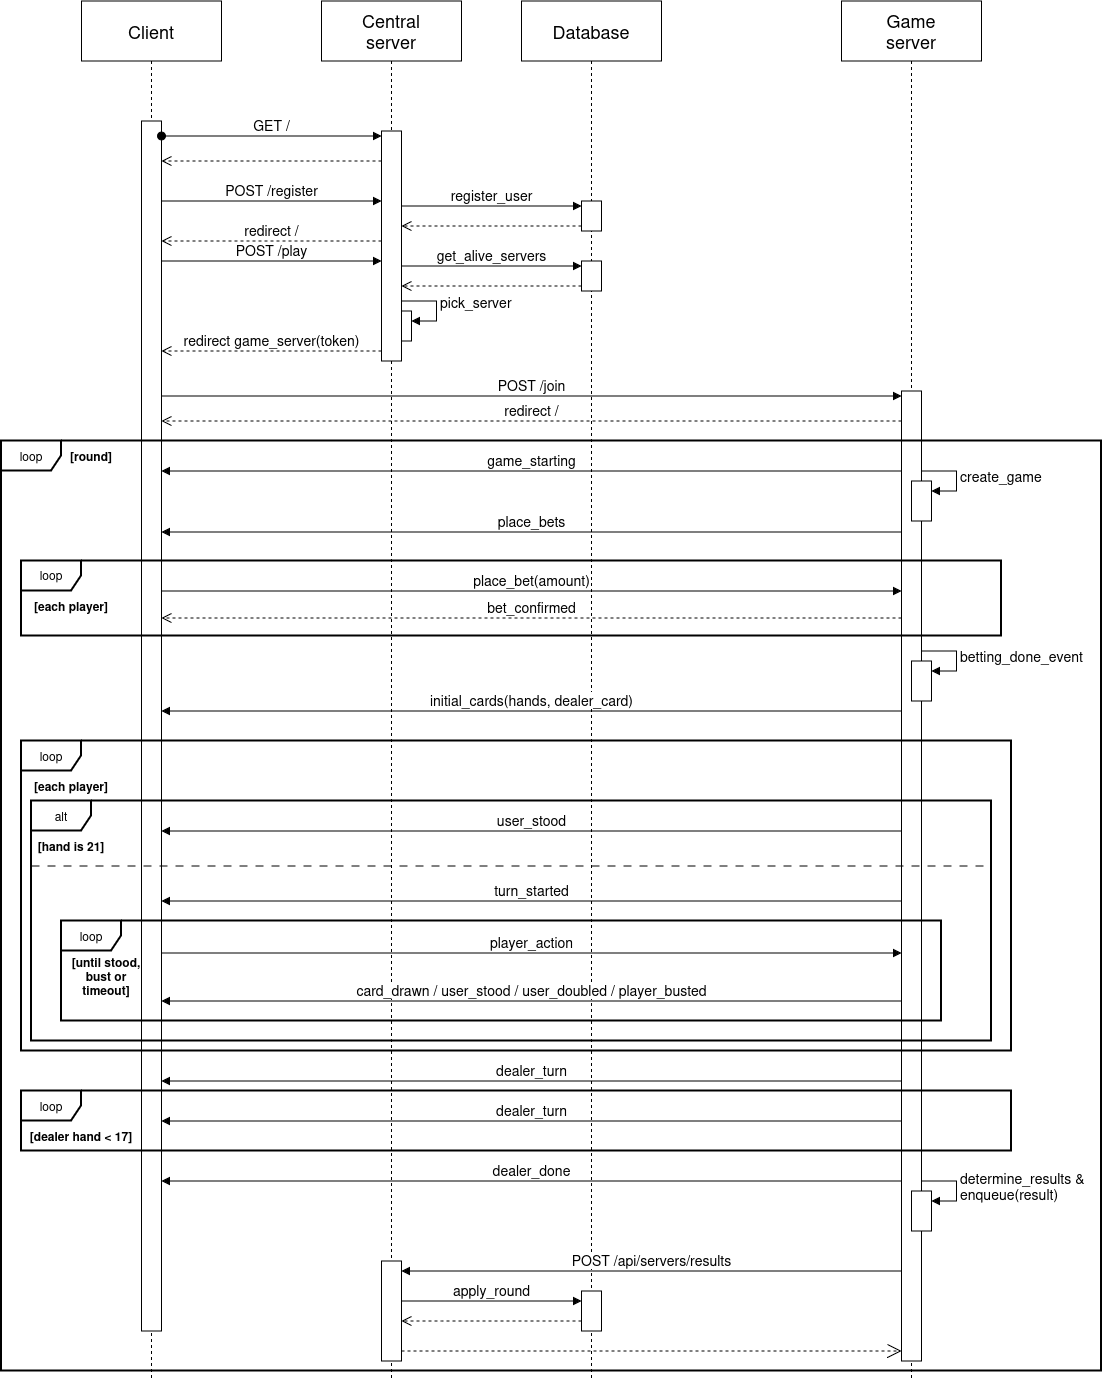
\includegraphics[width=1\textwidth]{img/sequence_diagram}
  \centering
  \caption{Interaction of the system during a game lifetime}
\end{figure}

\subsection{Behaviour}\label{behaviour}

% moved from ds-features, to be reworked
Game servers are multithread, and there is one thread per table.

\begin{itemize}
  \item how does \emph{each} component \textbf{behave} individually (e.g.~in \emph{response} to \emph{events} or messages)?
  \begin{itemize}
    \item some components may be \emph{stateful}, others \emph{stateless}
  \end{itemize}

  \item which components are in charge of updating the \textbf{state} of the system? \emph{when}? \emph{how}?
\end{itemize}

\begin{quote}
State diagrams are welcome here
\end{quote}

\subsection{Data and Consistency Issues}\label{data-and-consistency-issues}

% moved from ds-features, to be reworked
The balance is eventually consistent, and users are warned it may take a moment to update, so a stale number doesn't look like lost money.
One single instance of the database is shared across central server replicas, thus requiring coordination to handle race conditions.
For example, different dispatched may contend the player seat, player balance may be divided into multiple buy-ins, and the game server may post the results to different replicas over the lifespan of the buy-in and the seat.
The coordination is implemented through locks on the database. Rounds posts are parallel operations, that are handled at database level.
To ensure the concept of time is shared between replicas, therefore making leases handling equivalent, the database internal time is used. Database replication would further complicate time management.

\begin{itemize}
  \item Is there any data that needs to be stored?
  %
  \begin{itemize}
    \item \emph{what} data? \emph{where}? \emph{why}?
  \end{itemize}
  
  \item how should \emph{persistent data} be \textbf{stored}?
  %
  \begin{itemize}
    \item e.g.~relations, documents, key-value, graph, etc.
    \item why?
  \end{itemize}
  
  \item Which components perform queries on the database?
  %
  \begin{itemize}
    \item \emph{when}? \emph{which} queries? \emph{why}?
    \item concurrent read? concurrent write? why?
  \end{itemize}
  
  \item Is there any data that needs to be shared between components?
  %
  \begin{itemize}
    \item \emph{why}? \emph{what} data?
  \end{itemize}
\end{itemize}

\subsection{Fault-Tolerance}\label{fault-tolerance}

% moved from ds-features, to be reworked
The system values consistency and correctness more than availability. The game servers do not resume rounds after failures to avoid consistency risks, the user is warned the server is not responding and is kicked out. Bets of interrupted rounds are voided, so no money is lost, while results updates are persisted and are sent as soon as possible. Due to replication and the statelessness of the central servers, a crash of multiple instances only affects the load of the remaining. All game servers cycle the central servers as a failover mechanism and stop starting new rounds if none is reachable. The shared database and the client-side proxy are the single point of failure of the system. All the services are restarted upon crashes, in particular the game servers, as they may still have some unposted results.
Failure transparency is partial. If something goes wrong during a round, the user doesn't notice and the round finishes normally. If the central server can't be reached when the round ends, the user is warned and can't start a new round.
Data loss or corruption is prevented by combining at-least-once delivery with at-most-once recording, resulting in an exacly-once result application. The unapplied results ledger allows for troubleshooting when some results are rejected.

\begin{itemize}
  \item Is there any form of data \textbf{replication} / federation / sharing?
  %
  \begin{itemize}
    \item \emph{why}? \emph{how} does it work?
  \end{itemize}
  
  \item Is there any \textbf{heart-beating}, \textbf{timeout}, \textbf{retry mechanism}?
  %
  \begin{itemize}
    \item \emph{why}? \emph{among} which components? \emph{how} does it work?
  \end{itemize}
  
  \item Is there any form of \textbf{error handling}?
  %
  \begin{itemize}
    \item \emph{what} happens when a component fails? \emph{why}? \emph{how}?
  \end{itemize}
\end{itemize}

\subsection{Availability}\label{availability}

% moved from ds-features, to be reworked
The game servers can be scaled at run-time thanks to the registration mechanism, and they will be assigned some load by the central server dispatch.

\begin{itemize}
  \item Is there any \textbf{caching} mechanism?
  %
  \begin{itemize}
    \item \emph{where}? \emph{why}?
  \end{itemize}
  
  \item Is there any form of \textbf{load balancing}?
  %
  \begin{itemize}
    \item \emph{where}? \emph{why}?
  \end{itemize}

  \item In case of \textbf{network partitioning}, how does the system behave?
  %
  \begin{itemize}
    \item \emph{why}? \emph{how}?
  \end{itemize}
\end{itemize}

\subsection{Security}\label{security}

% moved from ds-features, to be reworked
Tokens signed with a shared secret are used to implement authentication and authorization in the system. The game and central servers share the symmetric key, the knowledge of the secret is what authenticates the entities. Authorization for servers is implemented by presenting the token on each request.
Users log in with their username and password, and the central server issues a join token when they want to play. This token authorizes them to the dispatched game server. The identity of the users and their money always come from the token, which is created and signed by a trusted source, instead of trusting the users.
Server and join token are not interchangeable and are told apart by a token field.
Traffic travels over unsecured connection, therefore the system is prone to replay attacks, eavesdropping and hijacking. The token expiry and the buy in management that seats the player only once bound the window for replay attacks.

\begin{itemize}
  \item Is there any form of \textbf{authentication}?
  %
  \begin{itemize}
    \item \emph{where}? \emph{why}?
  \end{itemize}

  \item Is there any form of \textbf{authorization}?
  %
  \begin{itemize}
    \item which sort of \emph{access control}?
    \item which sorts of users / \emph{roles}? which \emph{access rights}?
  \end{itemize}

  \item Are \textbf{cryptographic schemas} being used?
  %
  \begin{itemize}
    \item e.g.~token verification,
    \item e.g.~data encryption, etc.
  \end{itemize}
\end{itemize}

\section{Implementation}\label{implementation}

Please report here all the implementation (technology-dependent) choices you made while implementing your design.

\begin{quote}
  If you run out of time for this project, you may consider leaving some aspect unimplemented, 
  and simply discuss how you would have implemented them.
  %
  In this case, better would be to discuss unimplemented features in \cref{future-works}.
\end{quote}

% moved from ds-features, to be reworked
Communication happens with REST API and JSON data format between the servers, while WebSockets are used to communicate to the browser.

\begin{itemize}
  \item which \textbf{network protocols} to use?
  %
  \begin{itemize}
    \item e.g.~UDP, TCP, HTTP, WebSockets, gRPC, XMPP, AMQP, MQTT, etc.
  \end{itemize}
  
  \item how should \emph{in-transit data} be \textbf{represented}?
  %
  \begin{itemize}
    \item e.g.~JSON, XML, YAML, Protocol Buffers, etc.
  \end{itemize}
  
  \item how should \emph{databases} be \textbf{queried}?
  %
  \begin{itemize}
    \item e.g.~SQL, NoSQL, etc.
  \end{itemize}
  
  \item how should components be \emph{authenticated}?
  %
  \begin{itemize}
    \item e.g.~OAuth, JWT, etc.
  \end{itemize}

  \item how should components be \emph{authorized}?
  %
  \begin{itemize}
    \item e.g.~RBAC, ABAC, etc.
  \end{itemize}
\end{itemize}

\subsection{Technological details}\label{technological-details}

\begin{itemize}
  \item any particular \emph{framework} / \emph{technology} being exploited goes here
\end{itemize}

\section{Validation}\label{validation}

\subsection{Automatic Testing}\label{automatic-testing}

% moved from ds-features, to be reworked
Pytests ensure basic mechanisms are enforced.

\begin{itemize}
  \item how were individual components \textbf{\emph{unit}-test}ed?
  
  \item how was communication, interaction, and/or integration among components tested?
  
  \item how to \textbf{\emph{end-to-end}-test} the system?
  %
  \begin{itemize}
    \item e.g.~production vs.~test environment
  \end{itemize}

  \item for each test specify:
  %
  \begin{itemize}
    \item rationale of individual tests
    \item how were the test automated
    \item how to run them
    \item which requirement they are testing, if any
  \end{itemize}
\end{itemize}

\begin{quote}
recall that \emph{deployment} \textbf{automation} is commonly used to \emph{test} the system in \emph{production-like} environment
\end{quote}

\begin{quote}
recall to test corner cases (crashes, errors, etc.)
\end{quote}

\subsection{Acceptance test}\label{acceptance-test}

\begin{itemize}
  \item did you perform any \emph{manual} testing?
  %
  \begin{itemize}
    \item what did you test?
    \item why wasn't it automatic?
  \end{itemize}
\end{itemize}

\section{Deployment}\label{deployment}

% moved from ds-features, to be reworked
The system is configurable with .env variables.

\begin{itemize}
  \item should one install your software from scratch, how to do it?
  %
  \begin{itemize}
    \item provide instructions
    \item provide expected outcomes
  \end{itemize}

  \item what software should be installed on the machines to run your project? which versions?
  
  \item should one set environment variables or configuration files?
  
  \item if you're using containerization (e.g.~Docker), 
  describe how you engineered your deployment scrips (e.g. \texttt{docker-compose.yml} files)
\end{itemize}

\section{User Guide}\label{user-guide}

\begin{itemize}
  \item how to use your software?
  %
  \begin{itemize}
    \item provide instructions
    \item provide expected outcomes
    \item provide screenshots if possible
  \end{itemize}
\end{itemize}

\section{Self-evaluation}\label{self-evaluation}

\begin{itemize}
  \item An individual section is required for each member of the group
  \item Each member must self-evaluate their work, listing the strengths and weaknesses of the product
  \item Each member must describe their role within the group as objectively as possible.
\end{itemize}

It should be noted that each student is only responsible for their own section.

\section{Future works}\label{future-works}

% moved from ds-features, to be reworked
The system could need to be further expanded by introducing database replicas, new consistency mechanisms.
Updates to the servers require a restart, and there are no mechanism to safely shutdown the game servers, the round is interruped and bets are voided but money are not lost\NOTEside{this we can fix too}.

Discuss possible future works, improvements, extensions, optimizations, etc.

Also discuss here any unimplemented feature, and how you would have implemented it.

\bibliographystyle{plain}
\bibliography{references}

\end{document}